\documentclass[11pt,a4paper]{article}
\oddsidemargin 0.1 cm \evensidemargin 0.1cm \textwidth 16cm
\textheight24cm
\setlength{\topmargin}{0pt}\setlength{\headsep}{0pt}\pagestyle{empty}

\usepackage{graphicx}
\usepackage{variations}
\usepackage{enumerate}
\usepackage{amssymb}
\usepackage[latin1]{inputenc}  
\usepackage{fontenc}   
\usepackage{amsmath}
\usepackage{amsthm}
\usepackage{amsthm}
\usepackage{xypic}
\usepackage{variations}
%\usepackage{fancyhdr}
%\usepackage{xcolor}
%\usepackage{pstricks-add}
\usepackage[francais]{babel}
%\usepackage[french]{babel}
\newtheorem{defi}{D\'{e}finition}
\newtheorem{thm}{Th\'{e}or\`{e}me}
\newtheorem{rmq}{Remarque}
\newtheorem{prop}{Propri\'{e}t\'{e}}
\newtheorem{prop-def}{Propri\'{e}t\'{e}-D\'{e}finition}
\newtheorem{ex}{Exemple}
\newtheorem{exs}{Exemples}
\newtheorem{exer}{Exercice}
%\newtheorem{proof}{D\'{e}monstration}
\def\di{\displaystyle}
\newcommand{\vtab}{\rule[-0.4em]{0pt}{1.2em}}
\usepackage[top=0.5cm,bottom=0.5cm,right=1.5cm,left=1.5cm]{geometry}
\usepackage{pstricks,pst-plot} 
%\usepackage{framed}
\usepackage{amsmath}
%\usepackage{amssymb}
\usepackage{fancyhdr}
\usepackage{fancybox}
\usepackage{multicol}
%\usepackage{xcolor}
\usepackage{epsfig}
\usepackage{pifont}
%\usepackage[framed]{ntheorem}
%\usepackage[frenchb]{babel}
\usepackage{tabularx}
\def\R{{\mathbb R}}
\newtheorem{Rem}{Remarque}
\newcommand{\V}{\overrightarrow}
\newcommand{\Rep}{(O;\V{\imath};\V{\jmath})}
\newcommand{\Coor}[2]{\begin{pmatrix} #1\\#2 \end{pmatrix}}

\begin{document}
	\title{}         % Enter your title between curly braces
	\author{}        % Enter your name between curly braces
	\date{}          % Enter your date or \today between curly braces
	\maketitle
	
	\indent\vspace{-3cm}
	
	$$\fbox{\text{\Large{ Chapitre 1 - Feuille d'exercices n�3 : op�rations sur les vecteurs}}}$$
     
\hfill\\[0.2cm]
     

\noindent\underline{\textbf{Exercice 1 :}}\\[0.2cm]   % exercice 9 Barbazo 2014
Dans chacun des cas suivants, donner le r�sultat de la somme des vecteurs sous la forme d'un seul vecteur :
\begin{minipage}{0.3\linewidth}
\begin{enumerate}[$\diamond$]
\item $\V{AE}+\V{EG}$ ;
\item $\V{BF}+\V{AB}$ ;
\end{enumerate}
\end{minipage}
\begin{minipage}{0.3\linewidth}
\begin{enumerate}[$\diamond$]
\item $-\V{RS}+\V{RT}$ ;
\item $\V{AB}+\V{BA}$ ;
\end{enumerate}
\end{minipage}
\begin{minipage}{0.3\linewidth}
\begin{enumerate}[$\diamond$]
\item $\V{CM}-\V{CN}$ ;
\item $\V{EB}+\V{BP}+\V{PL}$.
\end{enumerate}
\end{minipage}
\hfill\\[0.5cm]

\noindent\underline{\textbf{Exercice 2 :}}\\[0.2cm]
Les segments $[KL]$ et $[RJ]$ ont le m�me milieu $I$.\\
Pour chaque proposition, dire si elle est vraie ou fausse ou si on ne peut pas savoir.\\
\begin{minipage}{0.35\linewidth}
\begin{enumerate}[$\diamond$]
\item $RL=KJ$ ;
\item $\V{RL}=\V{KJ}$ ;
\item $RJ=KL$ ;
\item $\V{LJ}=\V{KR}$ ;
\end{enumerate}
\end{minipage}
\begin{minipage}{0.55\linewidth}
\begin{enumerate}[$\diamond$]
\item $R$ est l'image de $L$ par la translation de vecteur $\V{KJ}$ ;
\item $\V{RK}+\V{JI}=\V{IK}$ ;
\item $\V{RI}=\di\frac{1}{2}\V{KL}$ ;
\item $\V{LK}=-2\V{KI}$.
\end{enumerate}
\end{minipage}
\hfill\\[0.4cm]


\noindent\underline{\textbf{Exercice 3 :}}\\[0.2cm]
$ABCD$ est un parall�logramme. Calculer :
$$\V{CD}+\V{AB}+\V{DA}+\V{DC}$$
Quelle remarque peut-on faire ?
\hfill\\

\noindent\underline{\textbf{Exercice 4 :}}\\[0.2cm]
On donne la figure ci-dessous :
$$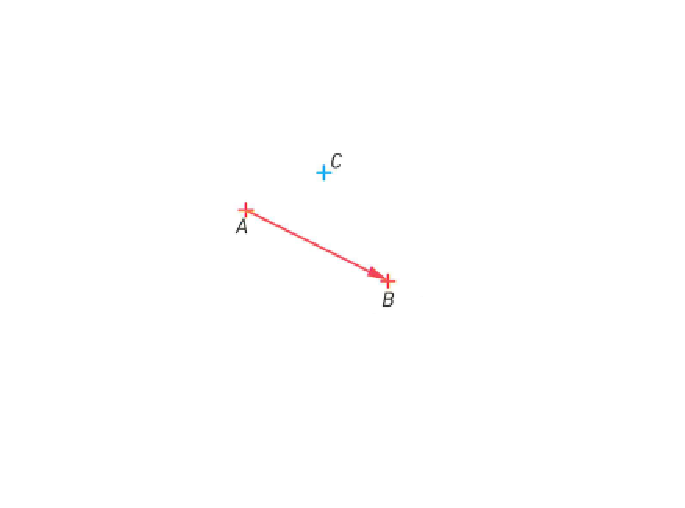
\includegraphics[scale=0.8]{exo-4.eps}$$
\begin{enumerate}
\item Construire le point $D$ tel que $\V{CD}=\V{AB}$.
\item Justifier que $\V{CA}=\V{DB}$.
\item Construire le point $E$ tel que $ABCE$ soit un parall�logramme.
\item Que dire des points $C$, $D$ et $E$. Justifier.
\item $F$ est l'image de $A$ par la translation de vecteur $\V{CB}$. Justifier que $\V{AC}=\V{FB}$.
\end{enumerate}	
\hfill\\

\newpage

\noindent\underline{\textbf{Exercice 5 : Vrai ou faux ?}}\\[0.2cm] % exo 24 Barbazo
Pour chaque proposition, dire si elle est vraie ou fausse.
\begin{enumerate}
\item Si $QFKG$ est un parall�logramme, alors $G$ est l'image de $Q$ par la translation de vecteur $\V{KF}$.
\item Si $\V{CH}=\V{RA}$, alors le quadrilat�re $CHRA$ est un parall�logramme.
\item Si $S$ est l'image de $B$ par la translation de vecteur $\V{NG}$, alors $\V{NB}=\V{GS}$.
\item Si $\V{KM}=\V{MD}$, alors $M$ est le milieu du segment $[KD]$.
\item Si $P$ a pour image $T$ par la translation de vecteur $\V{XW}$, alors $WPTX$ est un parall�logramme.
\item Si $C$ a pour image $D$ par la translation qui transforme $A$ en $B$, alors $[AD]$ et $[BC]$ ont le m�me milieu.
\end{enumerate}
\hfill\\

\noindent\underline{\textbf{Exercice 6 :}}\\[0.2cm] % exo 66 Barbazo
$ABCD$ est un rectangle. $I$ est le milieu de $[AB]$ et $E$ est le sym�trique de $I$ par rapport � $B$.
\begin{enumerate}
\item Placer le point $F$ tel que $\V{AF}=3\V{AD}$.
\item Que peut-on dire des points $C$, $E$ et $F$ ? Le d�montrer.
\end{enumerate}
\hfill\\

\noindent\underline{\textbf{Exercice 7 :}}\\[0.2cm] % exo 73 Barbazo
$ABCD$ est un parall�logramme. Les points $K$ et $L$ sont tels que $\V{BK}=-\di\frac{1}{2}\V{BA}$ et $\V{AL}=3\V{AD}$.
\begin{enumerate}
\item R�aliser une figure.
\item Que dire des points $K$, $C$ et $L$ ? Le d�montrer.
\end{enumerate}
\hfill\\

\noindent\underline{\textbf{Exercice 8 :}}\\[0.2cm] % exo 87 Barbazo
$ABC$ est un triangle quelconque. 
\begin{enumerate}
\item Construire le point $D$ tel que $\V{CD}=\V{CB}-2\V{AC}$.
\item D�montrer que $\V{BD}=2\V{CA}$.
\item Que peut-on en d�duire ?
\end{enumerate}
\hfill\\

\noindent\underline{\textbf{Exercice 9 :}}\\[0.2cm] % exo 94 Barbazo
Soit $ABCD$ un quadrilat�re et $M$ et $N$ les points d�finis par $\V{BM}=\di\frac{1}{2}\V{AB}$ et $\V{AN}=3\V{AD}$.
\begin{enumerate}
\item D�montrer que :
		\begin{enumerate}[$a.$]
		\item $\V{CM}=\di\frac{1}{2} \V{AB} - \V{BC}$ ;
		\item $\V{CN}=2\V{AD}-\V{DC}$.
		\end{enumerate}
\item En d�duire que si $ABCD$ est un parall�logramme, alors les points $C$, $M$ et $N$ sont align�s.
\end{enumerate}
\hfill\\


\noindent\underline{\textbf{Exercice 10 :}}\\[0.2cm] % exo 109 Barbazo
Soient $MNP$ et $MPC$ deux triangles �quilat�raux. 
\begin{enumerate}
\item D�montrer que $\V{MN}=\V{CP}$.
\item Construire les points $D$, $E$ et $F$ sym�triques respectifs de $N$, $P$ et $C$ par rapport � $M$.
\item D�montrer que $\V{CP}=\V{EF}$.
\item Compl�ter les �galit�s suivantes en n'utilisant que des noms de points pr�sents sur la figure :
		\begin{enumerate}[$a.$]
		\item $\V{MN}+\V{MP}= ... $ ;
		\item $\V{MN} + \V{MC} = ... $ ;
		\item $\V{MN}+\V{MC}+\V{ME} = ...$ ;
		\item $\V{MC} - \V{EM} = ... $ .
		\end{enumerate}
\item Exprimer $\V{ED}$ en fonction des vecteurs $\V{MN}$ et $\V{MP}$.
\end{enumerate}




\end{document}
